% This is samplepaper.tex, a sample chapter demonstrating the
% LLNCS macro package for Springer Computer Science proceedings;
% Version 2.20 of 2017/10/04
%
\documentclass[runningheads]{llncs}
%
\usepackage{graphicx}
\usepackage{float}
\usepackage{wrapfig}

% Used for displaying a sample figure. If possible, figure files should
% be included in EPS format.
%
% If you use the hyperref package, please uncomment the following line
% to display URLs in blue roman font according to Springer's eBook style:
% \renewcommand\UrlFont{\color{blue}\rmfamily}
\usepackage{color, colortbl}
\definecolor{navy}{RGB}{0,0,205}
\definecolor{darkred}{RGB}{178,34,34}
\definecolor{darkblue}{RGB}{0,10,230}
\definecolor{green}{RGB}{20,180,20}
\definecolor{verylightgray}{RGB}{220,220,220}

% colors fo rules
\definecolor{darkgreen}{RGB}{0,153,0}
\definecolor{darkorange}{RGB}{204,102,0}

\newcommand{\dollar}{\mbox{\textdollar}}
\definecolor{campusgold}{RGB}{194,142,14}
\definecolor{headlinegold}{RGB}{152, 112, 13}
\definecolor{coalgray}{RGB}{77,64,56}
\definecolor{moongray}{RGB}{186,168,146}
\definecolor{everblue}{RGB}{91,104,112}
\definecolor{slayterblue}{RGB}{124,166,192}
\definecolor{ameliablue}{RGB}{163,214,215}
\definecolor{landgreen}{RGB}{8,92,17}
\definecolor{rossgreen}{RGB}{132,158,42}
\definecolor{celerygreen}{RGB}{195,190,11}
\definecolor{springgreen}{RGB}{233,228,91}
\definecolor{oakenbrown}{RGB}{107,69,52}
\definecolor{bellbrick}{RGB}{199,108,20}
\definecolor{mackeyorange}{RGB}{255,155,26}
\definecolor{yellowwalk}{RGB}{255,209,0}
\definecolor{fountainteal}{RGB}{46,175,155}
\definecolor{pappyspurple}{RGB}{173,31,101}

\usepackage[round]{natbib}
\usepackage{amsmath}
\usepackage{stmaryrd}
\usepackage{amsfonts}
\usepackage{listings}
\lstdefinelanguage{Scala}%
{morekeywords={abstract,%
  case,catch,char,class,%
  def,else,extends,final,finally,for,%
  if,import,implicit,%
  match,module,%
  new,null,%
  object,override,%
  package,private,protected,public,%
  for,public,return,super,%
  this,%throw,throws,
  trait,try,type,throw,%
  val,var,%
  with,while,%
  yield,%
  },%
  sensitive,%
  morecomment=[l]//,%
  morecomment=[s]{/*}{*/},%
  morestring=[b]",%
  morestring=[b]',%
  showstringspaces=false%
  inputencoding=utf8,
  extendedchars=true,
  moredelim=[is][\overbar]{`}{`},
  moredelim=[is][\sout]{~}{~},
  escapechar=@
}[keywords,comments,strings]%

\definecolor{dkgreen}{rgb}{0,0.6,0}
\definecolor{gray}{rgb}{0.5,0.5,0.5}
\definecolor{mauve}{rgb}{0.58,0,0.82}
\definecolor{violet}{rgb}{0.53, 0.0, 0.69}
\definecolor{violet2}{rgb}{0.93, 0.51, 0.93}
\definecolor{backcolour}{rgb}{0.95,0.95,0.92}

\lstset{
  language=Scala,
  basicstyle=\ttfamily,
  keywordstyle={\bfseries\color{violet}},
  commentstyle=\color{dkgreen},
  stringstyle=\color{blue},
  mathescape
}
\usepackage[T1]{fontenc}
\usepackage[scaled=0.9]{beramono}

\makeatletter
\newcommand{\printfnsymbol}[1]{%
  \textsuperscript{\@fnsymbol{#1}}%
}
\makeatother

\begin{document}
%
\title{Wireframe2DOM: From Static Graph to Responsive HTML}
%
%\titlerunning{Abbreviated paper title}
% If the paper title is too long for the running head, you can set
% an abbreviated paper title here
%
\author{Shangyin Tan\thanks{equal contribution} \and
Tiger Tang\printfnsymbol{1}}
%
% First names are abbreviated in the running head.
% If there are more than two authors, 'et al.' is used.
%
\institute{Purdue University\\
\email{\{tan279,tang426\}@purdue.edu}}
%
\maketitle              % typeset the header of the contribution
%
\begin{abstract}
We propose a lightweight program synthesizer that generates HTML from static Wireframe design graph.
With our program, a UI/UX designer with little or no programming experience can obtain responsive HTML from design layout. 

\keywords{Program Synthesis  \and Web Development \and User Interface}
\end{abstract}
%
%
%
\section{Introduction}
Program synthesis community targets mainly on string processing and integer manipulating problem. However, the need for generating web application and other Graphical User Interface(GUI) applications is growing. While some UI/UX designers are capable of writing frontend code, providing them with a tool that generating HTML code can be beneficial. With HTML code equivalent to their interface design, designers can edit, test, and improve the original static layout. For example, many web applications now seek compatibility between PC and mobile devices. The different sizes complicate the designers' work. Some layouts are more promising on $16:9$ screen than on other smart devices. With the responsive HTML generated by our project, designer can preview the layout in a new resolution without re-drawing.

Our work focuses on configure the relationship between each atom elements in the static layout. We combine components of different sizes and locations into horizontal/vertical divisions and grids.  Instead of the absolute coordinate given by input, we assign margin to the converted structure and remember the relative position between them. Without the limitation of absolute coordinates, the converted structures can be rendered with the designers' true intention.

\section{Related work}
% Tiger

\section{Illustrative example}
% Shangyin
\section{Formal problem definition}
% Shangyin
In this work, we are given a list $L$, consisting of rectangles given their absolute coordinate with respective to origin. In addition, user provides the default size of the layout. All rectangles should be bounded by default size. Our objective is to find an equivalent HTML script which is: 
\begin{enumerate}
  \item \textbf{Precise -} Render the exact same layout when opened in  default size.
  \item \textbf{Responsive -} Automatically adjust the elements rendering if the browser is resized.
\end{enumerate}
\section{Preliminaries}
% Shangyin
\subsection{Workflow}
\begin{figure}[H]
  \vspace*{-0.1in}
  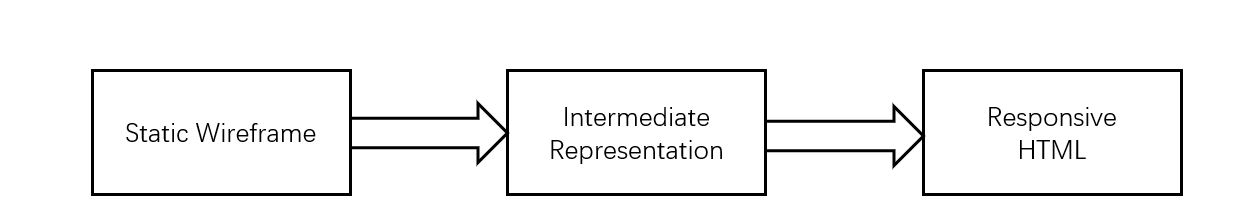
\includegraphics[width=1\textwidth]{src/workflow.JPG}
  \caption{Workflow}
\end{figure}
We define our workflow as a two-staged program. In the first stage, we synthesize the input Wireframe rectangles to IR. Then IR is compiled into universal HTML compatible with any browser in the second stage. 
\subsection{Input}
The input is defined as a list of rectangles, given their coordinates related to $(0,0)$, the upper-left corner of the canvas. For the consistency, we record the coordinates of the upper-left corner of a rectangle, as well as its width and height.
\subsection{IR Definition}
As discussed before, the intermediate presentation captures the nested hierarchy of raw rectangles. To maintain the hierarchical structure, we defined the data structure below.
\begin{figure}[H]
\vspace*{-0.2in}
\begin{lstlisting}[language=Scala,mathescape=true]
size = <Int, Int>
Div = <size>
HDiv = <size, VDiv*, Grid*, Div*>
VDiv = <size, HDiv*, Grid*, Div*>
Grid = <size, VDiv*, HDiv*, Div*>
Layout = Div | Grid | VDiv | HDiv
\end{lstlisting}
\caption{Definition of IR}
\end{figure}
We define \lstinline|Div| to be basic component of the hierarchy, which is equivalent to a raw rectangle in the input. All solid input rectangles are transformed into \lstinline|Div|s in different level of the tree in separate time during synthesizing. The three virtual containers for hierarchy are   \lstinline|HDiv|, \lstinline|VDiv|, \lstinline|GDiv|. As the name suggests, child containers of \lstinline|HDiv| and \lstinline|VDiv| are rendered in horizontal and vertical direction respectively. We define \lstinline|Grid| to behave like an HTML grid: two-dimensional container with auto row-wrapping. It contains homogenous elements, all rendered with same margin. 


\section{Algorithm}
% Shangyin
In this section, we explain the procedures we used synthesizing the list of rectangles to IR with an estimate order of time complexity. We also present the compilation process from IR to final HTML result.
\subsection{IR Synthesis}
Recall that the input is a list of rectangles. This is the starting point of the synthesis, and we target the nested hierarchical IR. 
\subsubsection{Cut}


\subsubsection{Input}
RECT\\
RECTLIST:= RECTLIST RECT | Nil
\subsubsection{IR}
DIV\\
HDIV:= HDIV|DIV|VDIV\\
VDIV:= HDIV|DIV|VDIV\\
First we divide the rectangles into section based on their $y$-axis. Then we use
greedy to find the earliest possible cut $y$ such that this $y$ does not divide any
other rects.


\section{Evaluation}
% Tiger
\section{Conclusion}
% Tiger

\end{document}